\documentclass[11pt,a4paper]{article}
\usepackage[final]{acl}
\usepackage[T5]{fontenc}
\usepackage[utf8]{inputenc}
\usepackage[english,vietnamese]{babel}
\usepackage{times,latexsym,microtype,inconsolata}
\usepackage{booktabs,array,tabularx}
\usepackage{amsmath,amssymb,graphicx,xcolor,tikz}
\usetikzlibrary{arrows.meta,positioning,shapes.geometric}
\hypersetup{hidelinks}
\setcitestyle{numbers,square,comma}
\makeatletter
\renewenvironment{thebibliography}[1]{%
  \section*{Tài liệu tham khảo}\phantomsection
  \addcontentsline{toc}{section}{Tài liệu tham khảo}\small
  \list{\@biblabel{\the\c@NAT@ctr}}{\@bibsetup{#1}\global\c@NAT@ctr\z@}%
  \let\p@NAT@ctr\@empty\renewcommand\theNAT@ctr{\arabic{NAT@ctr}}%
  \sloppy\clubpenalty4000\widowpenalty4000}{\endlist}
\makeatother
\newcommand{\unchecked}{\(\square\)}
\newcommand{\checked}{\(\boxtimes\)}
\newcommand{\code}[1]{{\small\texttt{\detokenize{#1}}}}
\setlength{\emergencystretch}{2em}

\title{Phát hiện phương tiện vượt đèn đỏ}
\author{Nguyễn Tuấn Anh \\
Lớp 124231 \\
Bài tập lớn môn Deep Learning}

\begin{document}
\maketitle
\pagestyle{plain}
\thispagestyle{plain}

\renewcommand{\abstractname}{Abstract}
\begin{abstract}
Bài báo trình bày hệ thống thị giác máy tính phát hiện phương tiện vượt đèn đỏ từ video camera giao thông cố định. Hệ thống kết hợp nhận diện phương tiện bằng YOLO, gán định danh theo thời gian bằng ByteTrack, phân loại trạng thái đèn và kiểm tra quỹ đạo cắt vạch dừng theo hướng di chuyển. Một sự kiện chỉ được xác nhận khi xe nằm trước vạch, cắt đoạn vạch hữu hạn trong trạng thái đèn đỏ và tiếp tục xuất hiện phía sau vạch đủ số khung hình quy định. Mỗi sự kiện được lưu cùng thời điểm, ID, ảnh toàn cảnh và ảnh cắt phương tiện. Detector được đánh giá trên tập con COCO gồm 1.000 ảnh train, 200 ảnh validation và 200 ảnh test với năm lớp giao thông. Trong cùng giao thức, YOLOv8s đạt mAP@0.50:0.95 là 0,318 và F1 là 0,529, cao nhất trong ba cấu hình SSD300-VGG16, YOLOv8s và YOLO11x; SSD300-VGG16 đạt tốc độ cao nhất, 166,8 FPS trên NVIDIA H100. Kết quả cho thấy YOLOv8s cân bằng tốt nhất giữa độ chính xác, tốc độ và độ phức tạp trên tập thử. Bài báo đồng thời phân tích giới hạn chuyển miền, sai số tích lũy và yêu cầu đánh giá ở mức sự kiện trước khi triển khai thực tế.
\end{abstract}

\section{Giới thiệu}
Vượt đèn đỏ có nguy cơ tạo xung đột trực tiếp tại nút giao. Giám sát thủ công nhiều luồng camera tốn nhân lực, khó bảo đảm tính nhất quán và thường chỉ cho phép xem lại sau sự cố. Một hệ thống tự động khoanh vùng sự kiện nghi vấn, giữ bằng chứng hình ảnh và xuất dữ liệu có cấu trúc sẽ hỗ trợ đáng kể cho người vận hành.

Bài toán không dừng ở nhận diện xe trong một ảnh. Hệ thống phải đồng thời xác định phương tiện nào đang được theo dõi, đèn nào điều khiển đúng làn, xe có thực sự đi qua vạch theo chiều bị giám sát hay không, và bằng chứng nào đủ để kiểm tra lại quyết định. Sai số của bất kỳ mô-đun nào cũng có thể lan truyền đến kết quả cuối. Mất ID có thể làm bỏ sót sự kiện; giữ trạng thái đỏ sau chuyển pha có thể tạo báo sai.

Đề tài xây dựng pipeline xử lý video hoàn chỉnh cho camera cố định. Các đóng góp chính gồm: (i) cấu hình hình học riêng cho từng video/camera bằng dấu vân tay nội dung; (ii) phát hiện cắt vạch có hướng trên đoạn thẳng hữu hạn; (iii) cơ chế xác nhận nhiều khung hình và xử lý trạng thái đèn không chắc chắn theo hướng thận trọng; (iv) báo cáo sự kiện có khả năng truy vết; và (v) thực nghiệm thống nhất so sánh ba detector trên cùng dữ liệu và phần cứng.

\section{Cơ sở lý thuyết và công trình liên quan}
\subsection{Nhận diện đối tượng}
YOLO định nghĩa nhận diện đối tượng như bài toán hồi quy hợp nhất từ ảnh đến hộp giới hạn và xác suất lớp, tạo nền tảng cho các detector một giai đoạn tốc độ cao \citep{redmon2016}. SSD cũng loại bỏ bước đề xuất vùng, sử dụng các hộp mặc định ở nhiều tỉ lệ và nhiều tầng đặc trưng để dự đoán lớp cùng độ lệch vị trí \citep{liu2016}. Hai hướng tiếp cận phù hợp với video giao thông, nơi thông lượng quan trọng bên cạnh độ chính xác.

Đề tài dùng SSD300-VGG16 làm baseline; YOLOv8s và YOLO11x đại diện cho hai cấu hình YOLO có quy mô khác nhau. Tập thử được trích từ COCO \citep{lin2014} và giữ năm lớp \textit{bicycle}, \textit{car}, \textit{motorcycle}, \textit{bus}, \textit{truck}.

\subsection{Theo dõi đa đối tượng}
Phát hiện độc lập từng frame không tạo định danh bền vững. ByteTrack liên kết quỹ đạo bằng cả các hộp có độ tin cậy thấp thay vì loại bỏ chúng ngay \citep{zhang2022}. Điều này hữu ích khi xe bị che khuất hoặc ở xa camera. Hệ thống dùng ByteTrack để nhận ID, rồi áp dụng logic cắt vạch trên chuỗi điểm neo của từng ID.

\subsection{Nhận diện trạng thái đèn}
Nhận diện đèn thường kết hợp phát hiện vùng đèn và phân loại màu. Kích thước nhỏ, chói sáng, ngược sáng và khác biệt thiết kế khiến chuyển miền trở thành thách thức \citep{pon2023}. Hệ thống dùng ROI đèn gắn với từng làn và MobileNetV2 của Autoware ở định dạng ONNX. MobileNetV2 sử dụng inverted residual và linear bottleneck để giảm chi phí tính toán \citep{sandler2018}. Khi không đủ tự tin, trạng thái được đưa về \code{UNKNOWN}, không suy diễn thành đỏ.

\section{Phát biểu bài toán}
Đầu vào là chuỗi frame $I_t$. Detector sinh tập
\begin{equation}
D_t=\{(b_i,c_i,p_i)\}_{i=1}^{n_t},
\end{equation}
với $b_i$ là hộp, $c_i$ là lớp và $p_i$ là độ tin cậy. Tracker ánh xạ mỗi quan sát sang ID $k$ và tạo quỹ đạo $\mathcal{T}_k=\{q_k^t\}$; $q_k^t$ là điểm neo giữa cạnh đáy hộp xe.

Mỗi làn được biểu diễn bởi cổng $G=(L,\boldsymbol{d},R,m)$ gồm đoạn vạch $L=(A,B)$, hướng hợp lệ $\boldsymbol{d}$, vùng đèn $R$ và hướng chuyển động $m$. Trạng thái đèn sau lọc thời gian là $s_t\in\{\text{RED},\text{YELLOW},\text{GREEN},\text{UNKNOWN}\}$. Với khoảng cách có dấu
\begin{equation}
\delta(q,L)=\frac{(B-A)\times(q-A)}{\lVert B-A\rVert_2},
\end{equation}
trong đó $\times$ là tích có hướng hai chiều.
ứng viên xuất hiện khi dấu của $\delta$ đổi theo chiều quy định và đoạn nối hai quan sát liên tiếp giao với chính đoạn $AB$. Sự kiện chỉ được xác nhận nếu $s_t=\text{RED}$ tại lúc cắt, xe tiếp tục ở phía sau vạch tối thiểu $K$ frame và khoảng cách lớn hơn biên $\epsilon$.

\section{Kiến trúc hệ thống}
\subsection{Pipeline tổng thể}
Hình~\ref{fig:pipeline} mô tả luồng xử lý. Camera được hiệu chỉnh một lần để xác định vạch, hướng đi và ROI đèn. Trong mỗi frame, hệ thống nhận diện phương tiện, cập nhật ID, phân loại đèn và hợp nhất kết quả tại bộ máy luật. Đầu ra gồm video, ảnh bằng chứng và báo cáo JSON/CSV/Markdown.

\begin{figure}[t]
\centering
\begin{tikzpicture}[
 node distance=3mm,
 block/.style={draw,rounded corners=2pt,align=center,text width=6.45cm,minimum height=6.5mm,font=\small},
 decision/.style={draw,diamond,aspect=4,align=center,font=\footnotesize,inner sep=1.4pt},
 arr/.style={-{Stealth[length=1.7mm]},thick}]
\node[block] (video) {Video / camera và cấu hình hình học};
\node[block,below=of video] (detect) {YOLO nhận diện xe, ByteTrack gán ID};
\node[block,below=of detect] (light) {ROI đèn, MobileNetV2 và lọc trạng thái};
\node[block,below=of light] (cross) {Quỹ đạo có hướng và giao đoạn vạch};
\node[decision,below=5mm of cross] (rule) {Đỏ tại lúc cắt và đủ xác nhận?};
\node[block,below=5mm of rule] (report) {Ảnh bằng chứng, video, JSON/CSV/Markdown};
\draw[arr] (video)--(detect); \draw[arr] (detect)--(light);
\draw[arr] (light)--(cross); \draw[arr] (cross)--(rule);
\draw[arr] (rule)--node[right,font=\footnotesize]{Có}(report);
\end{tikzpicture}
\caption{Pipeline phát hiện sự kiện vượt đèn đỏ.}
\label{fig:pipeline}
\end{figure}

\subsection{Hiệu chỉnh theo camera}
Cấu hình gồm hai đầu mút vạch, hộp đèn điều khiển và điểm chỉ hướng phía trước vạch. Nó được gắn với SHA-256 của video, kích thước frame và ID camera, tránh dùng nhầm tọa độ giữa các góc quay. Cách biểu diễn không giả định vạch ngang theo trục ảnh.

Hệ thống có mô-đun đề xuất vạch dựa trên Hough, hướng quỹ đạo, cụm xe dừng, độ dài và tương phản sơn, nhưng chỉ dùng thử nghiệm. Chế độ chính xác ưu tiên hình học do người dùng xác nhận vì vạch qua đường, mép đường và bóng sáng có thể giống vạch dừng.

\subsection{Nhận diện và theo dõi xe}
Detector giữ năm lớp phương tiện. Cấu hình video hiện tại dùng YOLO11x pretrained COCO, ảnh 960 và ngưỡng 0,10 để ByteTrack còn quan sát hộp yếu trong bước liên kết. Điểm neo mặc định $(0{,}5;1{,}0)$ tương ứng giữa cạnh đáy hộp.

Mỗi ID chỉ được ghi một lần trong một lượt chạy. Track mất quá 0,20 giây bị loại khỏi trạng thái chờ. Nếu mất quan sát đúng lúc cắt vạch, cả quan sát trước và sau khoảng trống đều phải ở đèn đỏ. Điều kiện này hạn chế suy diễn qua đoạn video thiếu bằng chứng.

\subsection{Trạng thái đèn}
ROI đèn được đặt riêng theo làn để tránh chọn nhầm đèn rẽ hoặc đèn của hướng giao cắt. Crop được chuẩn hóa về $224\times224$ và phân loại bởi MobileNetV2 với ngưỡng 0,80. Trạng thái mới phải lặp ba frame trước khi chấp nhận. Trong chuyển tiếp hoặc khi các đèn mâu thuẫn, đầu ra là \code{UNKNOWN}. Hệ thống không giữ \code{RED} khi mất tín hiệu; lựa chọn này có thể giảm recall nhưng tránh báo sai do trạng thái cũ bị kéo dài.

\subsection{Cắt vạch và xác nhận}
Thuật toán lưu vị trí cuối ở trước vạch cho từng cặp (ID, cổng). Khi điểm mới ở sau vạch, nó kiểm tra giao thật giữa đoạn quỹ đạo và đoạn vạch hữu hạn. Ứng viên đỏ phải duy trì phía sau vạch ba frame và vượt biên hai pixel. Nếu xe quay lại trước khi đủ xác nhận, ứng viên bị hủy.

Sự kiện lưu frame cắt, frame xác nhận, thời gian video, trạng thái đèn, ID cổng, ID xe, lớp, confidence và hai ảnh. Tách frame cắt khỏi frame xác nhận giữ đúng mốc thời gian thay vì gán thời điểm muộn do điều kiện nhiều frame.

\section{Cài đặt}
Hệ thống được hiện thực bằng Python, OpenCV, PyTorch/Ultralytics và ONNX Runtime. \code{main.py} điều phối pipeline; nhận diện đèn, cắt vạch, luật vi phạm, cấu hình cảnh và báo cáo được tách thành mô-đun. Mỗi lượt chạy có thư mục riêng, kèm cấu hình, hash checkpoint, số frame dự kiến, số frame đã xử lý và cờ hoàn tất.

\begin{table}[t]
\centering\small
\begin{tabularx}{\columnwidth}{@{}l>{\raggedright\arraybackslash}X@{}}
\toprule Thành phần & Thiết lập chính \\
\midrule
Xe & 5 lớp; confidence 0,10; ảnh 960 \\
Tracker & ByteTrack; mất tối đa 0,20 giây \\
Đèn & MobileNetV2 ONNX; confidence 0,80 \\
Ổn định đèn & Xác nhận trạng thái mới 3 frame \\
Cắt vạch & Giao đoạn có hướng; biên 2 pixel \\
Vi phạm & Đỏ tại lúc cắt; xác nhận 3 frame \\
Báo cáo & MP4, JSON, CSV, Markdown, JPEG \\
\bottomrule
\end{tabularx}
\caption{Cấu hình pipeline video.}
\label{tab:runtime}
\end{table}

Công cụ đánh giá sự kiện chỉ chấp nhận lượt chạy hoàn tất. Nó ghép một-một dự đoán và ground truth theo cổng với sai lệch thời gian tối đa 0,5 giây; dự đoán trùng được tính false positive.

\section{Thiết kế thực nghiệm}
\subsection{Dữ liệu và huấn luyện}
Tập con COCO gồm 1.000 ảnh train với 3.539 đối tượng, 200 ảnh validation với 685 đối tượng và 200 ảnh test với 762 đối tượng. Test không được dùng để chọn epoch hoặc siêu tham số. Ba mô hình dùng cùng thứ tự lớp và phép chia dữ liệu.

Mỗi mô hình được huấn luyện 80 epoch từ trọng số pretrained, seed 42. SSD300-VGG16 dùng ảnh $300\times300$, batch 8 và learning rate ban đầu 0,002. Hai YOLO dùng ảnh $640\times640$, batch 8 và cấu hình tối ưu mặc định. Checkpoint tốt nhất được chọn bằng mAP@0.50:0.95 trên validation.

\subsection{Chỉ số}
Độ chính xác hộp dùng COCO mAP@0.50:0.95 và mAP@0.50. Với confidence 0,25 và IoU 0,50:
\begin{align}
P&=\frac{TP}{TP+FP}, & R&=\frac{TP}{TP+FN},\\
F_1&=\frac{2PR}{P+R}.&&
\end{align}
Tốc độ được đo batch 1, FP32 trên NVIDIA H100 sau warm-up và đồng bộ CUDA, gồm tiền xử lý model, suy luận và NMS nhưng không gồm đọc video, tracking hay ghi báo cáo. FPS vì vậy là tốc độ detector, không phải tốc độ đầu-cuối.

\section{Kết quả và đánh giá}
\subsection{So sánh định lượng}
Bảng~\ref{tab:results} cho thấy YOLOv8s đạt cao nhất ở mAP, precision, recall và F1. So với SSD, mAP@0.50:0.95 tăng 0,061 điểm tuyệt đối và F1 tăng 0,084 điểm. YOLO11x có mAR100 cao nhất nhưng thấp hơn YOLOv8s ở mAP và F1.

\begin{table*}[t]
\centering\small
\begin{tabular}{@{}lrrrrrrrr@{}}
\toprule
Mô hình & mAP50--95 & mAP50 & mAR100 & Precision & Recall & F1 & FPS & Tham số (M) \\
\midrule
SSD300-VGG16 & 0,257 & 0,433 & 0,385 & 0,544 & 0,385 & 0,445 & \textbf{166,8} & 24,3 \\
YOLOv8s & \textbf{0,318} & \textbf{0,519} & 0,460 & \textbf{0,570} & \textbf{0,497} & \textbf{0,529} & 119,9 & \textbf{11,1} \\
YOLO11x & 0,309 & 0,513 & \textbf{0,474} & 0,554 & 0,484 & 0,514 & 65,2 & 56,9 \\
\bottomrule
\end{tabular}
\caption{Kết quả trên 200 ảnh test; P/R/F1 dùng confidence 0,25 và IoU 0,50.}
\label{tab:results}
\end{table*}

\begin{figure*}[t]
\centering
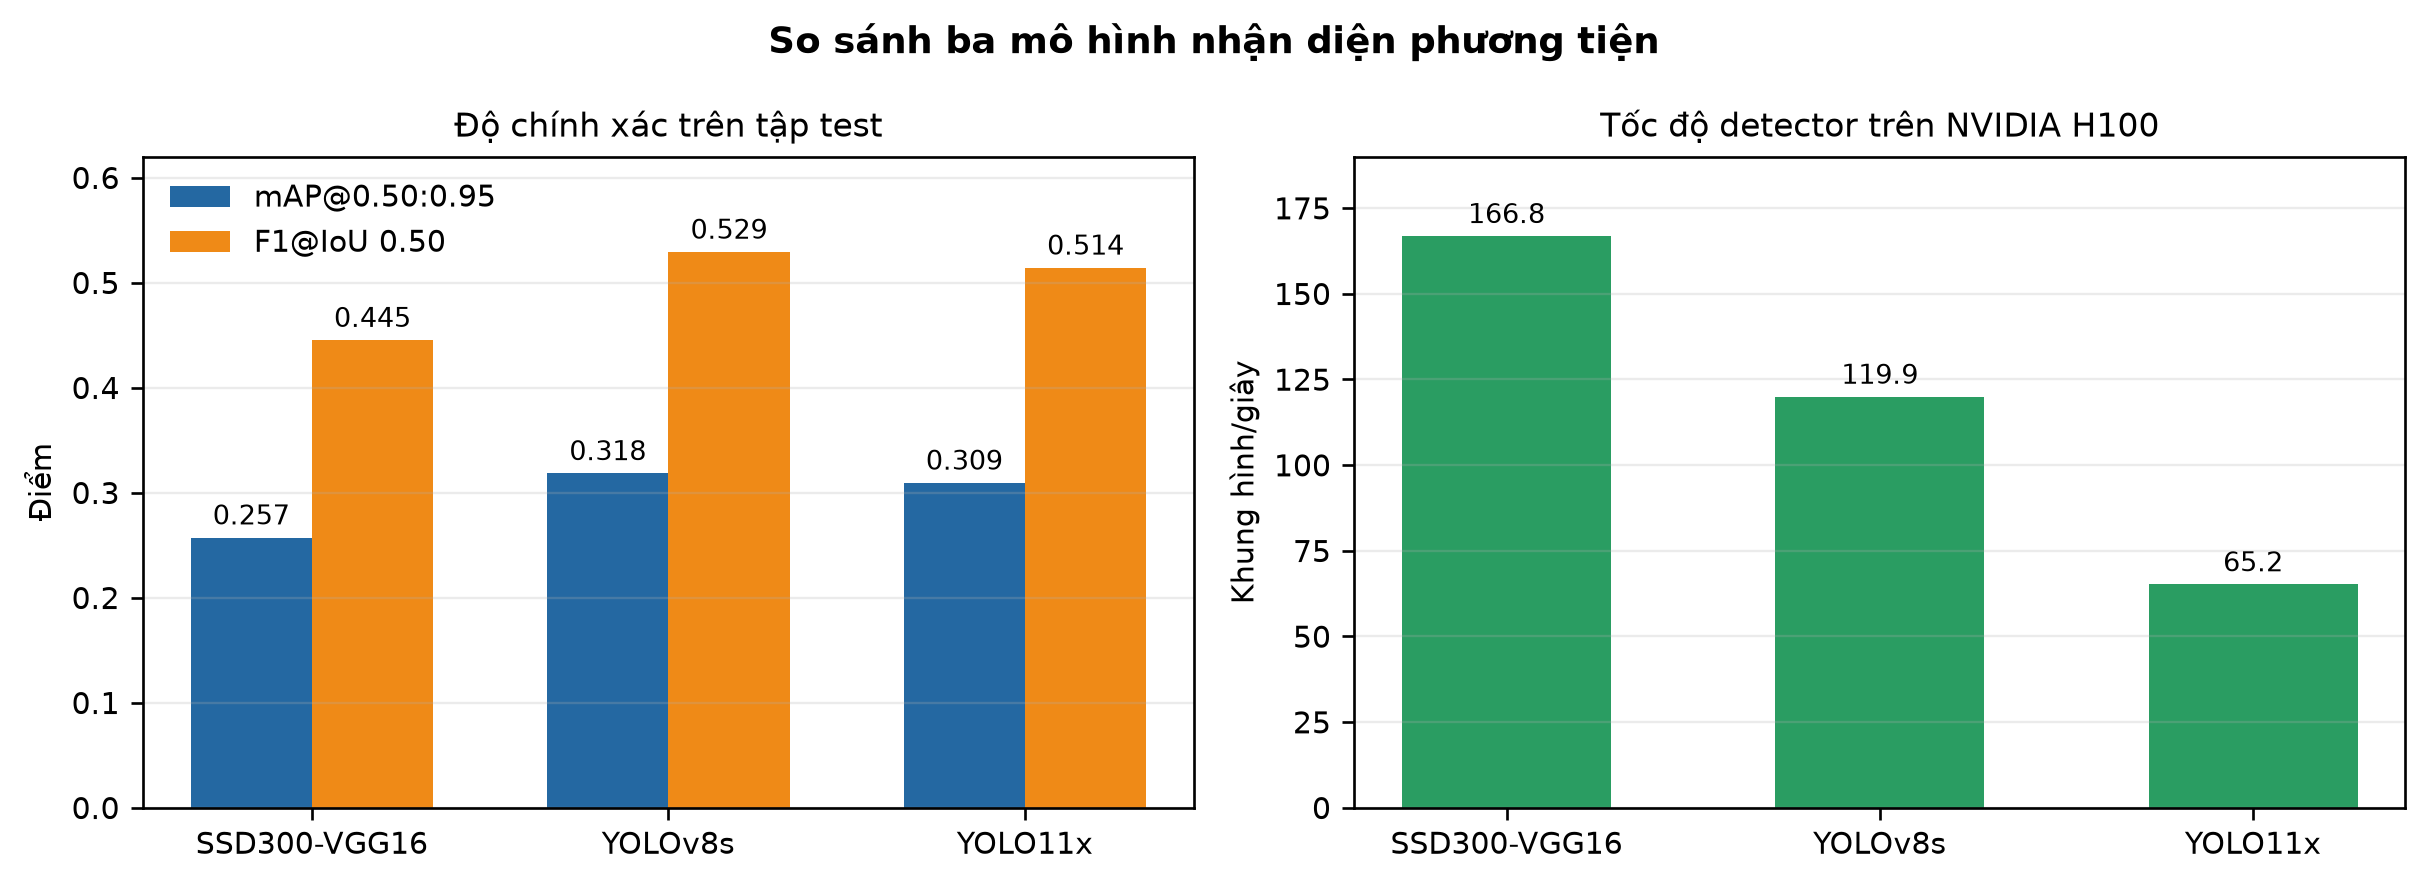
\includegraphics[width=0.98\textwidth]{figures/model_comparison.png}
\caption{So sánh độ chính xác và tốc độ. YOLOv8s dẫn đầu về mAP và F1; SSD nhanh nhất.}
\label{fig:model-comparison}
\end{figure*}

SSD nhanh hơn YOLOv8s khoảng 39,1\% nhưng giảm chất lượng hộp. YOLO11x có tham số gấp khoảng 5,1 lần YOLOv8s, trong khi mAP thấp hơn 0,009 và tốc độ chỉ bằng 54,3\%. Quy mô lớn hơn không mang lại lợi ích tương ứng trên tập hiện tại.

\begin{figure}[t]
\centering
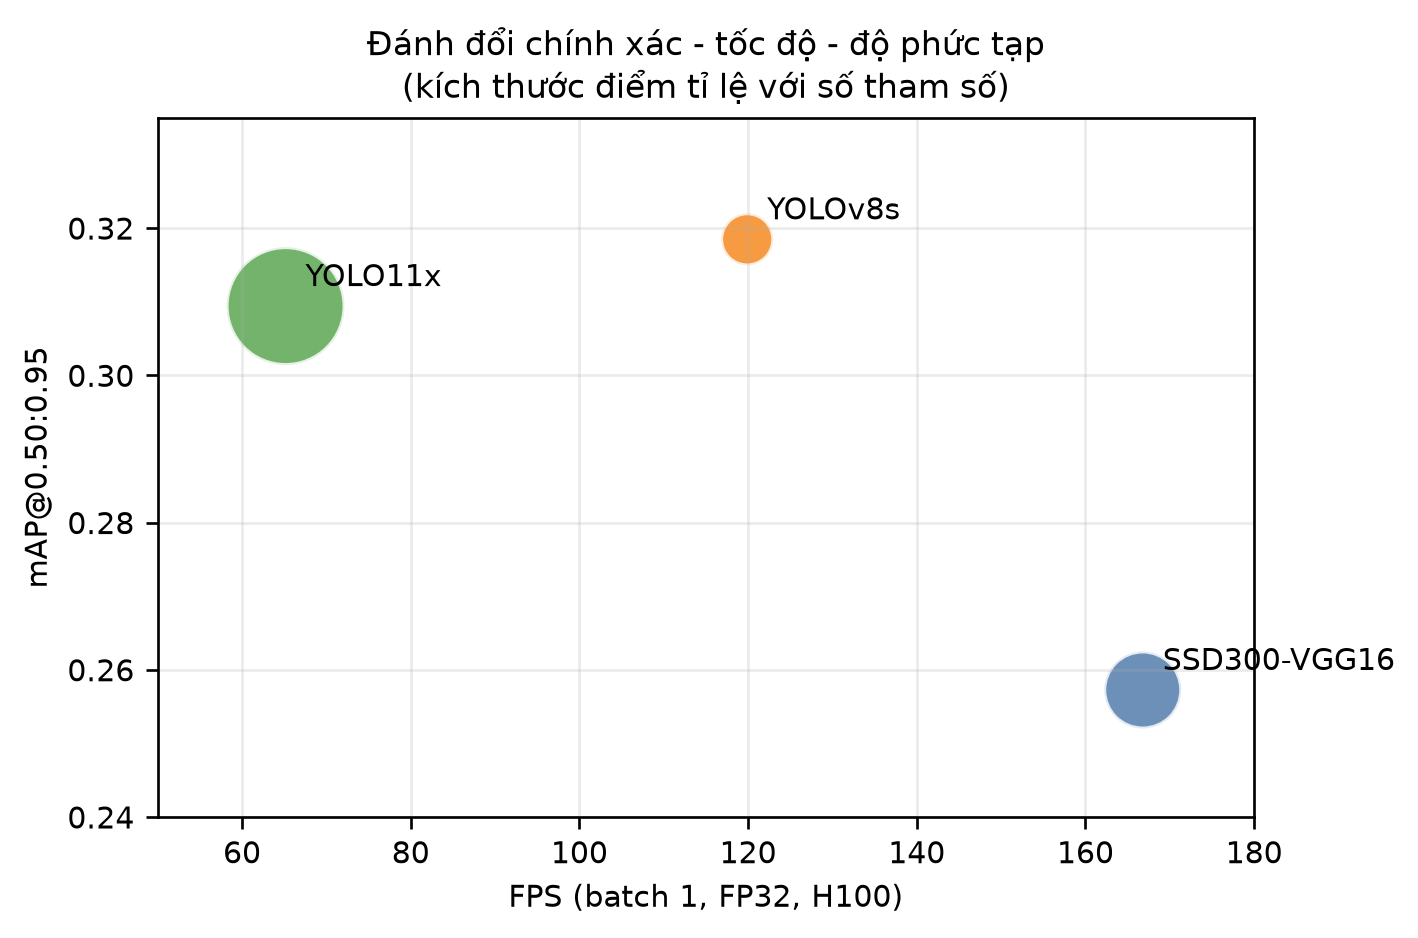
\includegraphics[width=\columnwidth]{figures/accuracy_speed_tradeoff.png}
\caption{Đánh đổi chính xác--tốc độ; kích thước điểm tỉ lệ số tham số.}
\label{fig:tradeoff}
\end{figure}

YOLOv8s nằm gần biên tối ưu thực dụng: mAP cao nhất, 119,9 FPS và 11,1 triệu tham số. Tuy nhiên, pipeline video hiện dùng YOLO11x pretrained COCO vì kiểm tra trực quan ở camera mục tiêu cho thấy checkpoint tùy biến nhỏ có thể sinh hộp giả trên mặt đường trống. Quyết định triển khai phải dựa trên dữ liệu camera được gán nhãn, không chỉ tập con COCO.

\subsection{Chi phí huấn luyện}
YOLOv8s huấn luyện trong 9,2 phút, checkpoint 21,5 MB và peak VRAM 2.654 MB. SSD cần 16,4 phút, checkpoint 92,6 MB và 1.090 MB. YOLO11x cần 27,4 phút, checkpoint 109,1 MB và 7.348 MB. YOLOv8s đồng thời có checkpoint nhỏ nhất và thời gian huấn luyện ngắn nhất.

Đây là so sánh cấu hình thực dụng, không phải thí nghiệm cô lập kiến trúc: kích thước đầu vào, augmentation và tối ưu giữa SSD và YOLO khác nhau. Kết quả chỉ mô tả các cấu hình đã chạy.

\subsection{Đánh giá định tính sự kiện}
Hình~\ref{fig:sequence} minh họa hệ thống duy trì ID, gắn trạng thái đỏ, kiểm tra xe tiến qua vạch và chỉ đổi nhãn sau đủ xác nhận. Việc hiển thị vạch, ROI làn, hộp, ID và đèn giúp phát hiện lỗi hình học hoặc liên kết.

\begin{figure}[t]
\centering
\includegraphics[width=\columnwidth]{figures/crossing_sequence.jpg}
\caption{Chuỗi frame theo dõi và xác nhận xe cắt vạch khi đèn đỏ. Số vàng là chỉ số frame; vạch đỏ là cổng giám sát.}
\label{fig:sequence}
\end{figure}

Trong lượt chạy hoàn tất trên \code{red1.mp4}, hệ thống xử lý đủ 203/203 frame ở 30 FPS và tạo hai sự kiện \code{confirmed\_red\_crossing}. Sự kiện đầu cắt ở frame 56, xác nhận frame 58, confidence 0,77; sự kiện sau cắt ở frame 89, xác nhận frame 91, confidence 0,89. Độ trễ hai frame phù hợp điều kiện ba quan sát liên tiếp tính cả frame ứng viên.

\begin{figure}[t]
\centering
\begin{minipage}[t]{0.48\columnwidth}
\centering\includegraphics[width=\linewidth]{figures/violation_evidence_1.jpg}
\scriptsize (a) ID 15, 1,833 giây.
\end{minipage}\hfill
\begin{minipage}[t]{0.48\columnwidth}
\centering\includegraphics[width=\linewidth]{figures/violation_evidence_2.jpg}
\scriptsize (b) ID 25, 2,933 giây.
\end{minipage}
\caption{Ảnh bằng chứng của hai sự kiện. Khung đỏ đánh dấu phương tiện cần kiểm tra; toàn cảnh giữ ngữ cảnh đèn và nút giao.}
\label{fig:evidence}
\end{figure}

Ảnh toàn cảnh quan trọng vì crop xe không chứng minh được trạng thái đèn, hướng đi hay quan hệ với vạch. Hai sự kiện này là đầu ra vận hành cần kiểm tra, chưa phải ground truth độc lập; không thể tự suy ra precision hoặc recall toàn hệ thống.

\section{Phân tích sai số và hạn chế}
Detector có thể bỏ sót xe nhỏ, xe che khuất hoặc nhầm bóng. Tracker có thể đổi ID sau che khuất dài. Classifier đèn chịu ảnh hưởng bởi chói sáng, mưa, đèn mũi tên và khác biệt khu vực. Vạch sai vài pixel có thể đổi frame cắt; chọn nhầm cổng hoặc hướng làm luật sự kiện mất ý nghĩa.

Các kiểm soát hiện tại giảm nhưng không loại bỏ sai số. \code{UNKNOWN} hạn chế báo sai do đèn mơ hồ; giao đoạn hữu hạn loại quỹ đạo cắt phần kéo dài ngoài làn; xác nhận nhiều frame loại dao động gần vạch; dấu vân tay video ngăn dùng nhầm cấu hình. Ảnh bằng chứng và log hỗ trợ kiểm tra phần còn lại.

Thí nghiệm detector chỉ dùng một seed và tập con COCO nhỏ nên chưa có khoảng tin cậy. COCO không đại diện đầy đủ cho mật độ xe máy, kiểu đèn, thời tiết và camera Việt Nam. Các chỉ số hộp chưa đo độ ổn định ID, màu đèn, sai số vạch hay chất lượng sự kiện. Mô hình Autoware chủ yếu học từ đèn Nhật Bản; confidence cao trên vài crop không đồng nghĩa accuracy cao tại camera mục tiêu. FPS H100 cũng không phản ánh máy phổ thông và không gồm toàn pipeline.

Đánh giá tiếp theo cần gán thủ công toàn bộ sự kiện trên video test, kể cả xe detector bỏ sót và video không vi phạm. Mỗi nhãn chứa ID cổng và thời điểm cắt theo cùng quy ước điểm neo. Dữ liệu phải chia theo camera/video, không chia ngẫu nhiên frame lân cận. Cần bổ sung ban đêm, mưa, ngược sáng, ùn tắc, xe máy và che khuất. Các mô-đun nên được đo riêng bằng mAP, confusion matrix đèn, IDF1/HOTA và sai số thời điểm cắt trước khi đánh giá đầu-cuối.

\section{Kết luận}
Bài báo trình bày hệ thống phát hiện phương tiện vượt đèn đỏ có kiến trúc mô-đun, hình học có hướng và bằng chứng truy vết. YOLOv8s đạt cân bằng tốt nhất trên tập con COCO: mAP@0.50:0.95 bằng 0,318, F1 bằng 0,529 và 119,9 FPS với 11,1 triệu tham số. SSD nhanh nhất nhưng kém chính xác; YOLO11x lớn hơn đáng kể mà không cải thiện mAP.

Giá trị chính của hệ thống nằm ở việc hợp nhất nhận diện, theo dõi, trạng thái đèn và quỹ đạo thành quyết định sự kiện có bằng chứng. Tuy nhiên, chỉ số detector chưa đủ để khẳng định độ chính xác toàn pipeline. Hướng tiếp theo là xây dựng dữ liệu camera thực tế, gán nhãn sự kiện độc lập, đánh giá theo camera giữ kín và tối ưu cho điều kiện giao thông Việt Nam.

\begin{thebibliography}{9}
\bibitem{redmon2016} Joseph Redmon, Santosh Divvala, Ross Girshick và Ali Farhadi. 2016. You Only Look Once: Unified, Real-Time Object Detection. Trong \textit{CVPR}, trang 779--788. \url{https://arxiv.org/abs/1506.02640}.
\bibitem{liu2016} Wei Liu, Dragomir Anguelov, Dumitru Erhan và cộng sự. 2016. SSD: Single Shot MultiBox Detector. Trong \textit{ECCV}, trang 21--37. \url{https://arxiv.org/abs/1512.02325}.
\bibitem{lin2014} Tsung-Yi Lin, Michael Maire, Serge Belongie và cộng sự. 2014. Microsoft COCO: Common Objects in Context. Trong \textit{ECCV}, trang 740--755. \url{https://arxiv.org/abs/1405.0312}.
\bibitem{zhang2022} Yifu Zhang, Peize Sun, Yi Jiang và cộng sự. 2022. ByteTrack: Multi-Object Tracking by Associating Every Detection Box. Trong \textit{ECCV}, trang 1--21. \url{https://arxiv.org/abs/2110.06864}.
\bibitem{sandler2018} Mark Sandler, Andrew Howard, Menglong Zhu, Andrey Zhmoginov và Liang-Chieh Chen. 2018. MobileNetV2: Inverted Residuals and Linear Bottlenecks. Trong \textit{CVPR}, trang 4510--4520. \url{https://arxiv.org/abs/1801.04381}.
\bibitem{pon2023} Alex D. Pon và cộng sự. 2023. Traffic Light Recognition using Convolutional Neural Networks: A Survey. \textit{arXiv:2309.02158}. \url{https://arxiv.org/abs/2309.02158}.
\bibitem{autoware2026} Autoware Foundation. 2026. Traffic Light Classifier for Autoware: Model Card. \url{https://huggingface.co/AutowareFoundation/traffic_light_classifier}.
\end{thebibliography}

\section*{Lời cảm ơn}
Em xin trân trọng cảm ơn thầy cô giảng dạy môn Deep Learning đã cung cấp nền tảng kiến thức và định hướng để em thực hiện đề tài \textit{Phát hiện phương tiện vượt đèn đỏ}. Em cũng xin cảm ơn cộng đồng mã nguồn mở và các tác giả của những công trình được trích dẫn.

\clearpage
\onecolumn
\renewcommand{\contentsname}{Mục lục}
\tableofcontents

\clearpage
\section*{Tuyên bố sử dụng AI}
\begin{enumerate}
  \item Sử dụng AI hỗ trợ viết báo cáo:\\
        \checked\ Yes \qquad \unchecked\ No.
  \item Sử dụng AI hỗ trợ sinh các biểu đồ:\\
        \checked\ Yes \qquad \unchecked\ No.
  \item Sử dụng AI hỗ trợ sinh giao diện:\\
        \unchecked\ Yes \qquad \checked\ No.
  \item Sử dụng AI hỗ trợ sinh test cases:\\
        \checked\ Yes \qquad \unchecked\ No.
  \item Sử dụng bao nhiêu \% AI: \textbf{70\%}.
\end{enumerate}

\end{document}
